\documentclass[10pt]{article}
%les packages et leurs options
\usepackage[a4paper, textheight=22cm, right=3cm, heightrounded]{geometry}
\usepackage[utf8]{inputenc} 	%les accents français
\usepackage[T1]{fontenc}        %encodage clavier français
\usepackage[inline]{asymptote}  
\usepackage[english]{babel}   	%typo et césures françaises
\usepackage{amsmath, amsfonts, amsthm, amssymb}	% les maths
\usepackage{enumerate}		%listes enrichies
\usepackage{graphicx}           %insertion de figures
\usepackage{xcolor}
\usepackage{color,colortbl}
\usepackage{listingsutf8}       %intégration utf8 dans listing
\usepackage{calc}
\usepackage{multicol}
\usepackage{tabularx}           %pour des tableaux sur mesures
\usepackage{tabulary}
\usepackage{import}             %pour une seule compilation à partir de
                                %l'ensemble des sources
%\usepackage{frcursive}         %une fonte cursive
\usepackage[ %captio et sa personnalisation
labelfont={small,bf},textfont=it,figurename=Fig,
%le compteur fig repart à 0 à chaque nouveau chapitre
%lorsque la légende ne contient qu'une seule ligne
%elle doit tenir compte de la justification
figurewithin=section,singlelinecheck=false,
%Alignement à gauche
justification=raggedright]{caption}

%%%% Des figures sans label juste un numéro%%%%%%%%
%On modifie le label de la légende
%\DeclareCaptionFormat{Fig}{\begin{cursive}Fig #2\end{cursive}} 
%\captionsetup{captionformat=Fig,labelsep=quad}
%On change la couleur du label
%\DeclareCaptionFont{gray}{\color{gray}}
%\captionsetup{labelfont={gray,bf}}
%%%%%%%%%%%%%%%%%%%%%%%%%%%%%%%%%%%%%%%%%%%%%%%%%%%
\usepackage{floatrow} %floatrow et sa personnalisation
\floatsetup{style=plain,capposition=TOP} 
\usepackage[Lenny]{fncychap} %Mise en page des chapitres

%Définition d'un nouveau langage(asy) pour listing
\definecolor{bckgcolor}{rgb}{0.9,0.9,0.8}
\definecolor{keywordstc}{rgb}{0.7,0,0}
\definecolor{comments}{rgb}{0,0,1}
\lstdefinelanguage{asy}
                  {morekeywords={arrowbar, path, draw, label, real, pair,
                      picture, ticks, pen, bool, void},
                    sensitive=false,
                    morecomment=[l][\color{comments}]{//},
                    morecomment=[s]{/*}{*/},
                    morestring=[b]"
                  }
 \lstset{
   frameround=tttt,
   frame=single,
   numbers=left,
   language=asy, 
   numberstyle=\tiny,stepnumber=1, 
   basicstyle=\scriptsize\ttfamily,
   keywordstyle=\color{keywordstc}, 
   numbersep=5pt,
   tabsize=2,
   backgroundcolor=\color{bckgcolor}
}
%%%%%%%%%%%%%%%%%%%%%%%%%%%%%%%%%%%%%
% Majuscules droites en mode math %%%
%%%%%%%%%%%%%%%%%%%%%%%%%%%%%%%%%%%%%
\DeclareMathVersion{majDroites}
\DeclareSymbolFont{majuscules}{OML}{cmm}{m}{it}
\SetSymbolFont{majuscules}{majDroites}{OT1}{cmr}{m }{n}
\DeclareMathSymbol{A}{\mathalpha}{majuscules}{"41}
\DeclareMathSymbol{B}{\mathalpha}{majuscules}{"42}
\DeclareMathSymbol{C}{\mathalpha}{majuscules}{"43}
\DeclareMathSymbol{D}{\mathalpha}{majuscules}{"44}
\DeclareMathSymbol{E}{\mathalpha}{majuscules}{"45}
\DeclareMathSymbol{F}{\mathalpha}{majuscules}{"46}
\DeclareMathSymbol{G}{\mathalpha}{majuscules}{"47}
\DeclareMathSymbol{H}{\mathalpha}{majuscules}{"48}
\DeclareMathSymbol{I}{\mathalpha}{majuscules}{"49}
\DeclareMathSymbol{J}{\mathalpha}{majuscules}{"4A}
\DeclareMathSymbol{K}{\mathalpha}{majuscules}{"4B}
\DeclareMathSymbol{L}{\mathalpha}{majuscules}{"4C}
\DeclareMathSymbol{M}{\mathalpha}{majuscules}{"4D}
\DeclareMathSymbol{N}{\mathalpha}{majuscules}{"4E}
\DeclareMathSymbol{O}{\mathalpha}{majuscules}{"4F}
\DeclareMathSymbol{P}{\mathalpha}{majuscules}{"50}
\DeclareMathSymbol{Q}{\mathalpha}{majuscules}{"51}
\DeclareMathSymbol{R}{\mathalpha}{majuscules}{"52}
\DeclareMathSymbol{S}{\mathalpha}{majuscules}{"53}
\DeclareMathSymbol{T}{\mathalpha}{majuscules}{"54}
\DeclareMathSymbol{U}{\mathalpha}{majuscules}{"55}
\DeclareMathSymbol{V}{\mathalpha}{majuscules}{"56}
\DeclareMathSymbol{W}{\mathalpha}{majuscules}{"57}
\DeclareMathSymbol{X}{\mathalpha}{majuscules}{"58}
\DeclareMathSymbol{Y}{\mathalpha}{majuscules}{"59}
\DeclareMathSymbol{Z}{\mathalpha}{majuscules}{"5A}
\mathversion{majDroites} 


%les macros et le reste
%% Version de la macro figAsy utilisant minipage et listings
%%%%                  debut macro                       %%%%
\newcommand{\figAsy}[5]
{\noindent
\begin{minipage}[c]{0.4\textwidth}
\begin{figure}[H]
\ffigbox[\FBwidth]
{\includegraphics[width=#1, height=#2]{#3.pdf}}
{\caption{\label{#5}\footnotesize #4}}
\end{figure}
\end{minipage}
\hfill
\begin{minipage}[c]{0.55\textwidth}
 \tiny
   \lstinputlisting[inputencoding=utf8/latin1,tabsize=7]{#3.asy}
 \normalsize
\end{minipage}
\vspace{0.5cm}
}
%% La même macro mais avec la possibilité d'indiquer la plage de ligne
%% à afficher.
\newcommand{\figAsyLine}[6]
{
\begin{minipage}[c]{0.45\textwidth}
\begin{figure}[H]
\ffigbox[\FBwidth]
{\includegraphics[width=#1, height=#2]{#3.pdf}}
{\caption{\footnotesize #4}}
\end{figure}
\end{minipage}
\hfill
\begin{minipage}[c]{0.55\textwidth}
 \tiny
   \lstinputlisting[inputencoding=utf8/latin1,firstline=#5,lastline=#6]{#3.asy} 
 \normalsize
\end{minipage}
\vspace{0.5cm}
}

%% La macro pour insérer uniquement le code%%%%%%%%%%%%%%%%%%%%%%
\newcommand{\code}[2]
{
\begin{center}
\begin{minipage}{#1}
\lstinputlisting[inputencoding=utf8/latin1]{#2.asy}  
\end{minipage}
\end{center}
}

%%Définition de la numérotation des subsection%%%%%%%%%%%
\renewcommand{\thesubsubsection}{\alph{subsubsection}.}
%%%%                   fin macro                         %%%%

\usepackage{wallpaper}
\usepackage{hyperref}
\hypersetup{
 backref=true,       %permet d'ajouter des liens dans... 
 pagebackref=true,   %...les bibliographies
 hyperindex=true,	 %ajoute des liens dans les index. 
 colorlinks=true,    %colorise les liens
 breaklinks=true,
       %permet le retour à la ligne dans les liens trop longs 
 urlcolor= blue,     %couleur des hyperliens
 linkcolor= blue,    %couleur des liens internes
 bookmarks=true,     %créé des signets pour Acrobat 
 bookmarksopen=true, %si les signets Acrobat sont créés,
                     %les afficher complètement. 
}

\begin{document}
%\listoffigures
\thispagestyle{empty}
\ULCornerWallPaper{1}{couverture-en.pdf}
.
\newpage
\ClearWallPaper
\tableofcontents
\newpage

\section{Introduction}
The asy-circuit package is a collection of graphical elements for drawing electrical circuits. Asy-circuit also offers the ability to create complex graphical components called sub-circuits (assembly of electrical components in series and parallel) with the same properties as the basic components. This feature allows you to dynamically extend the limits of the design of an electrical circuit as needed.
    I want to give special thanks jpreve for his early interest in this work, for his advice and for the constructive discussions we have had.
\section{Basics}
\subsection{Components}
{\color{gray}{\subsubsection{Using components}}}

Each component has a list of properties that are set at the time of his statement by assigning values to their corresponding parameters. Let's start by analyzing the pattern of resistance.\par

\figAsy{6cm}{1.5cm}{./asytopdf/exo1}{Resistor}{exo1} 

On \emph{line 4} we find a \verb|Resistor(R)| type \verb|Element|. The creation of components for all type \verb|Element| components always uses the following format:\par

\begin{center}
\verb|Element e = Name_of_component(components_parameters);|
\end{center}
The string \verb|"R"| is the text label associated with the component. You will find below a list of other existing settings. We shall see later that each \verb|Element|, or electrical component, has in addition to its basic characteristics, functions which allow the user to access, modify or supplement the parameters assigned at the initialization of the electrical component\\
On \emph{line 5} are the circuit points between which the resistance is drawn.\\
Finally on \emph{line 6} the function \verb|join()| draws the ohmic conductor (\verb|Resistor|) between points A and B.

\figAsy{6cm}{1.2cm}{./asytopdf/exo2}{Resistors}{exo2} 
  
The code in \emph{Fig} \ref{exo2} shows another way to declare the components. They may be initialized directly by using the function \verb|join ()|. (On one hand this function makes the code more compact. On the other hand it deprives the user of some of  the advantages given by the declaration of an \verb|Element|. Further down this will be explained in detail.Now let's consider the list of available parameters during the initialization of a electrical component.\\
\begin{center}
\begin{minipage}{0.8\linewidth}
\begin{lstlisting}
  pair center=(0,0), real size=1,
  real angle=0, pen fillpen=invisible,
  pen drawpen=currentpen ... Label[] L
\end{lstlisting}
\end{minipage}
\end{center} 
\begin{description}
\item[center] position of the center of the element in user coordinates
\item[size] component size, the value of this parameter represents the magnification factor applied to the component. If you specify \verb|size=2|, the component will be twice as large.
\item[angle] angle of rotation of the element in relation to the direction of the wire
\item[fillpen] fill in color when possible. This parameter cannot be used on a coil, for example.
\item[drawpen]  stroke color
\item[L] label text, for the moment we can not add a single label but we can precisely choose its position around the electrical component.
\end{description}

{\color{gray}{\subsubsection{Using parameters}}}
Here are two examples to highlight the use of the different parameters.

\figAsy{6cm}{1.5cm}{./asytopdf/exo3}{Parameters}{exo3}

To place a label at a specific location around the electrical component you can use the \verb|align| parameter of the function \verb|Label()| already present in asymptote. This parameter receives a value (type \emph{pair}) indicating the position relative to the electrical component for example S for South, or what amounts to the same (0, -1). The other predefined values are N for North, E for East and W for West. The combinations SW, 2SW are also possible but you can write 0.3S +1.2 N + (0.4,0.2) as well.

\figAsy{6cm}{1.5cm}{./asytopdf/exo3_1}{A bit of fantasy in this rectangular world }{exo3_1}

{\color{gray}{\subsubsection{Components list}}}
The list below is far from complete, it will be enriched based on times and needs.

\figAsy{6cm}{1cm}{./asytopdf/zresistor}{Resistor}{zresistor} 

\figAsy{6cm}{1cm}{./asytopdf/capacitor}{Capacitor}{capacitor} 

\figAsy{6cm}{1cm}{./asytopdf/coil}{Coil}{coil} 

\figAsy{6cm}{1.5cm}{./asytopdf/battery}{Battery}{battery} 

\figAsy{6cm}{1.5cm}{./asytopdf/gen}{ideal generator}{gen} 

\figAsy{6cm}{1.5cm}{./asytopdf/icc}{Current generator}{icc} 

\figAsy{6cm}{1cm}{./asytopdf/diode}{Diode}{diode} 

\figAsy{6cm}{1cm}{./asytopdf/zener}{Zener}{zener}

\figAsy{6cm}{1.8cm}{./asytopdf/motor}{Motor}{motor} 

\figAsy{6cm}{1.2cm}{./asytopdf/lampe}{Lamp}{lampe}  

\figAsy{6cm}{1.5cm}{./asytopdf/sw}{Switch}{sw} 

\figAsy{6cm}{1.5cm}{./asytopdf/pot}{Potentiometer}{pot} 

\figAsy{6cm}{1.5cm}{./asytopdf/tr}{PNP et NPN}{tr} 

\figAsy{6cm}{1.5cm}{./asytopdf/oa}{Operational Amplifier}{oa} 

\figAsy{6cm}{1.5cm}{./asytopdf/tsw}{Interrupteur}{tsw} 

\figAsy{6cm}{1.5cm}{./asytopdf/tension}{Tension}{tension} 

\figAsy{6cm}{1.5cm}{./asytopdf/i}{Electrical current}{i} 

\figAsy{6cm}{1.5cm}{./asytopdf/ground}{Ground}{ground} 

\figAsy{6cm}{1.5cm}{./asytopdf/var}{Variable symbol}{var} 


\subsection{Using the \texttt{join()} function}
\begin{center}
\verb|join(pair A, pair B, bool dot=true ...Element[] e)|
\end{center}
\begin{itemize}
\item \verb|A|: starting point
\item \verb|B|: end point
\item \verb|dot|: marks with a red dot the ends A and B
\item \verb|e|: list of electrical components
\end{itemize}
\bigskip
If nothing is indicated for the component then the function \verb|join()| calculates and automatically place the elements (components).In other words, the elements are placed so that the amount of wire on either side is roughly constant. But rest assured it is quite possible to indicate the exact position of an element between two points A and B. Remember that I said from the outset that an \emph{Element} has features that enrich the basic parameters. Well the time has come to describe these features in detail. These functions are actually called \textbf{methods}. To indicate the precise position of an electrical component we use the method \verb|setPosition(real a)| where \verb|a| is the relative position between two terminals A and B on the wire. There \verb|a=0| is for A and \verb|a=1| is for B, we show for example \verb|a=0.5| to place the component in the center of [AB], which is the function \verb|join()| by default. In the following example we will move our components to the ends of the segment [AB]. 

\figAsy{6cm}{1.5cm}{./asytopdf/exo4}{Method setPosition(real a)}{exo4}

As you can see the syntax is very simple once the component is declared --- \emph{lines~4 and 6} --- just follow the name of the component \verb|r| or \verb|b| for a point and method name --- \emph{line~5} and \emph{line~7}~--- indicating the value(s) of the method parameter(s).\\
Note that the method \verb|join()| directs the segment [AB]. As you can see in the following example, it is not quite equivalent to draw the components from A to B or vice versa.

\figAsy{6cm}{4cm}{./asytopdf/exo4_1}{A to B}{exo4_1}

\figAsy{6cm}{4cm}{./asytopdf/exo4_2}{B to A}{exo4_2}

At the completion of an electrical circuit it may be necessary to pay attention to the orientation of the branches of electrical circuit. Asymetrical components such as the diode, have an additional argument, \verb|int type=0|, to allow the easy reversal of the pole connection. The argument \verb|type| has two values:
\begin{itemize}
    \item 0 default
    \item And one to reverse the connection of the poles - rotate 180 degrees.
\end{itemize}

\figAsy{6cm}{4cm}{./asytopdf/exo4_3}{B to A, with the diode in the other direction}{exo4_3}

\subsection{The methods of an element}

If the electrical component is initialized directly by using the method \verb|join()| the components is referred to as an \emph{anonymous} \emph{Element} and the user cannot access its methods.\\
Using the methods of an \emph{Element} is possible only in case the component is declared as:
\begin{center}
\verb|Element e = ...|
\end{center}

This provides the following methods:
\begin{enumerate}
\item \verb|setPosition(real a)|
\item \verb|addTension(int type=0, Label L, real decal=1.2, real multlength=1, pen p=black)|
\item \verb|addLabel(Label L, real rot=90)|
\item \verb|variable(real length=1,real rot=45,pen p=currentpen)|
\item \verb|connect(int n=0)|
\end{enumerate}

{\color{gray}{\subsubsection{setPosition}}}
See the code used in example \ref{exo4}.

{\color{gray}{\subsubsection{addTension}}}
This method adds a voltage arrow across an electrical component. It accepts the following parameters.

\begin{enumerate}
\item \verb|type| (0 ou 1) to indicate the direction of the arrow
\item \verb|L| text label for the voltage arrow
\item \verb|decal| distance between the component and the voltage arrow
\item \verb|multlength| fixed length of the voltage arrow
\item \verb|p| to use the pen
\end{enumerate}
The following two examples will help you understand the various parameters of this method.

\figAsy{6cm}{2cm}{./asytopdf/exo5}{Method addTension()}{exo5}

\figAsy{6cm}{2cm}{./asytopdf/exo6}{Method addTension()}{exo6}

{\color{gray}{\subsubsection{addLabel}}}
There may seem to be some redundancy between this method and the parameter \verb|L| of a component, but as I said in the introduction, this package allows the user to manufacture complex components dynamically (by association several basic components). It will then be possible to comment with a text label, an \verb|Element| created for the needs of the circuit.
\begin{center}
\includegraphics{asytopdf/parallel.pdf}
\end{center}
In this example we will describe the code a little later, after each bypass circuit is actually a sub-type circuit of the type \verb|Element| and for each sub circuit the method \verb|addLabel()| may be applied.

{\color{gray}{\subsubsection{variable}}}
This method is used to indicate that the value of a component is adjustable by the user.

\figAsy{6cm}{4cm}{./asytopdf/exo7}{Method variable()}{exo7} 

{\color{gray}{\subsubsection{connect}}}
The \verb|connect()| method allows the connection of electrical components with more than two terminals. The method \verb|join()| is reserved for dipoles.

\figAsy{4cm}{4cm}{./asytopdf/exo8}{Method connect()}{exo8} 

\emph{Line 5} allows the placement of the component by using the parameter \verb|Center|. \emph{Line 6} draws the component, it is the function draw () which replaces the function \verb|join()|.\\
In \emph{line 7} we retrieve the coordinates of the base, collector and transmitter which are then stored in a series of points. All that's remains is to use these points to draw our electric system.

\vspace{.5cm}
\section{Electric circuits}
\subsection{Assistance in drawing}
To make drawing more easily electrical circuits, asy-cir offers the use of a dot-grid display with the the help of the function
\begin{center}
\begin{minipage}{0.8\linewidth}
\begin{lstlisting}
addGrid(picture pic=currentpicture,
	     int x=(int)max(currentpicture).x,
	     int y=(int)max(currentpicture).y,
	     int griddivx=10,
	     int griddivy=10,
	     pen pen=black);
\end{lstlisting}
\end{minipage}
\end{center}

\begin{itemize}
\item \verb|x| width of the grid. 
\item \verb|y| height of the grid. 
\item The next two parameters correspond to the number of divisions in \verb|x| and \verb|y|.
\item \verb|pen| color of the grid.
\end{itemize}

\figAsy{5cm}{5cm}{./asytopdf/grille}{Number of division by default : 10}{grille} 

\figAsy{5cm}{5cm}{./asytopdf/grille2}{5 divisions on x and y}{grille2} 

The coordinates in red indicate the step of the grid
\noindent 
\newpage
\subsection{Examples of circuits}
{\color{gray}{\subsubsection{Kirchhoff}}}
\figAsy{5.7cm}{5.7cm}{./asytopdf/kirchoff}{Kirchhoff}{kirchoff} 
\vspace{2cm}
{\color{gray}{\subsubsection{Simple}}}
\figAsy{5.7cm}{4cm}{./asytopdf/lamp}{Lamps}{lamp} 
\newpage
{\color{gray}{\subsubsection{Connection of a transistor}}}
\figAsy{5.7cm}{5cm}{./asytopdf/transistor}{Transistor}{transistor} 
\vspace{2cm}
{\color{gray}{\subsubsection{Circuit star}}}
\figAsy{5cm}{5cm}{./asytopdf/etoile}{Star}{etoile} 
\newpage
{\color{gray}{\subsubsection{Electric circuits with ground}}}
\figAsy{5cm}{5cm}{./asytopdf/tension1}{Ground and draw()}{tension1} 

\section{How to draw a complex Element?}
With asy-circ, it is possible to create a new element by using the combination of basic components in series and in parallel. The type \emph{element} of this association, which could be described as sub-circuit or \emph{super Element}, and will thus allow the use the methods of an Element.
For this purpose we use the object \verb|circuit()| which accepts a parameter list Element.\\
\begin{center}
\verb|Element e = Circuit(...Element[] e)|
\end{center}
The construction of a sub-circuit is accomplished in the following two way:\\
\begin{enumerate}
\item \verb|serie(real decal=20)|
\item \verb|parallel(real decal=10, real hc=0, int branch=1)|
\end{enumerate}
\subsection{series and parallel electric circuits}
Start with a series circuit. The method accepts a single parameter series decal. It allows the user to set the spacing between the various components.\\

\figAsy{6cm}{1.5cm}{./asytopdf/resistor}{Series}{resistor} 

The \verb|parallel| method accepts three parameters
\begin{enumerate}
\item \verb|decal| secures the vertical space between two components
\item \verb|branch| to select the branch that is connected to the rest of the circuit. By default the connection is on the lowest branch that bears the number 1, the number of next branch is 2 and so on.
\item \verb|hc| adds an offset to shift the branch connection. To connect to the middle of two branches write hc = decal / 2.\\
\end{enumerate}

\figAsy{6cm}{3cm}{./asytopdf/resistor2}{Parallel}{resistor2} 

\subsection{customize sub-circuit}
Some examples that will help you understand how to apply the methods of an element to a sub-circuit.

\figAsy{5.5cm}{4cm}{./asytopdf/resistor1}{Series and parralel}{resistor1} 

We can construct relatively complex sub-circuits with a minimum of code. Note that the use of sub-circuits can limit connecting points and the function \verb|join()|.

\figAsy{7cm}{7cm}{./asytopdf/resistor3}{Series and parallel}{resistor3}

\section{For fun}
\subsection{Asy-circ and mechanics}
Now, two simulations in mechanics. I leave you the pleasure to imagine many others.

\figAsy{6cm}{5cm}{./asytopdf/fun1}{Oscillations}{fun1}

\figAsy{6cm}{3cm}{./asytopdf/fun2}{Oscillations on an inclined plane}{fun2}

\subsection{Unusual examples}
All examples were made with asym-circ.\\
\begin{center}
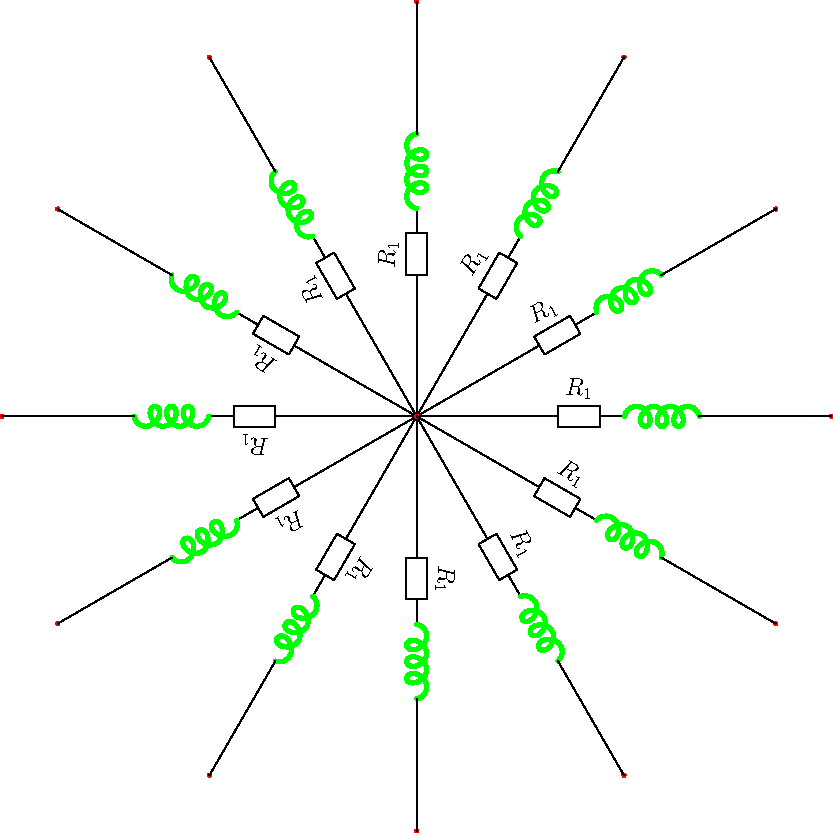
\includegraphics[scale=.8]{./asytopdf/insolite0.pdf}
\end{center}

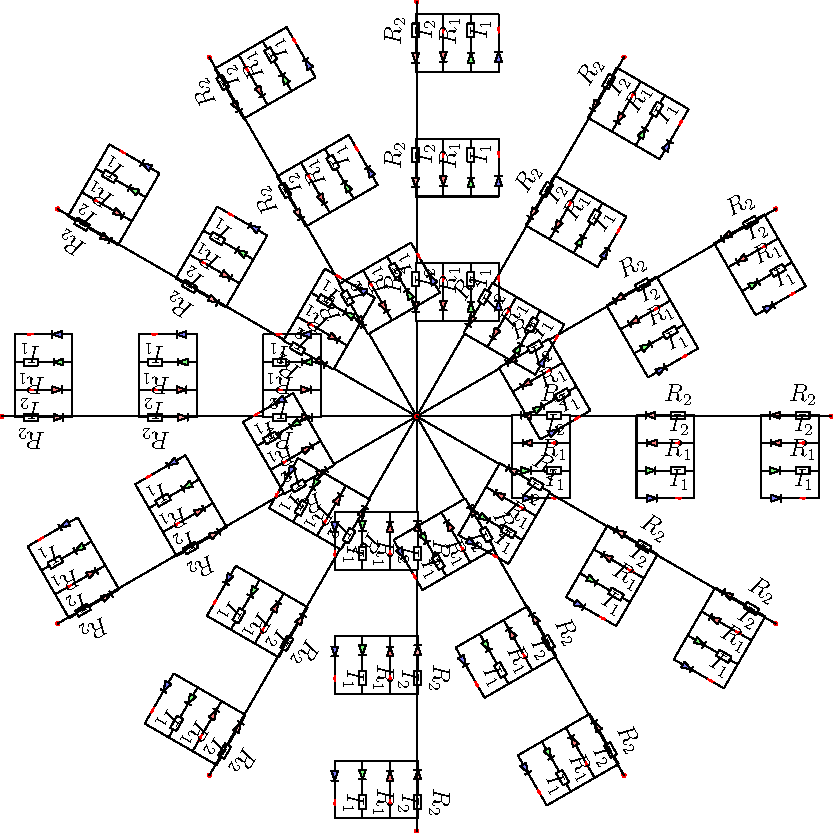
\includegraphics[scale=.5]{./asytopdf/insolite1.pdf}
\hfill\includegraphics[scale=.6]{./asytopdf/resistor4.pdf}

\begin{center}
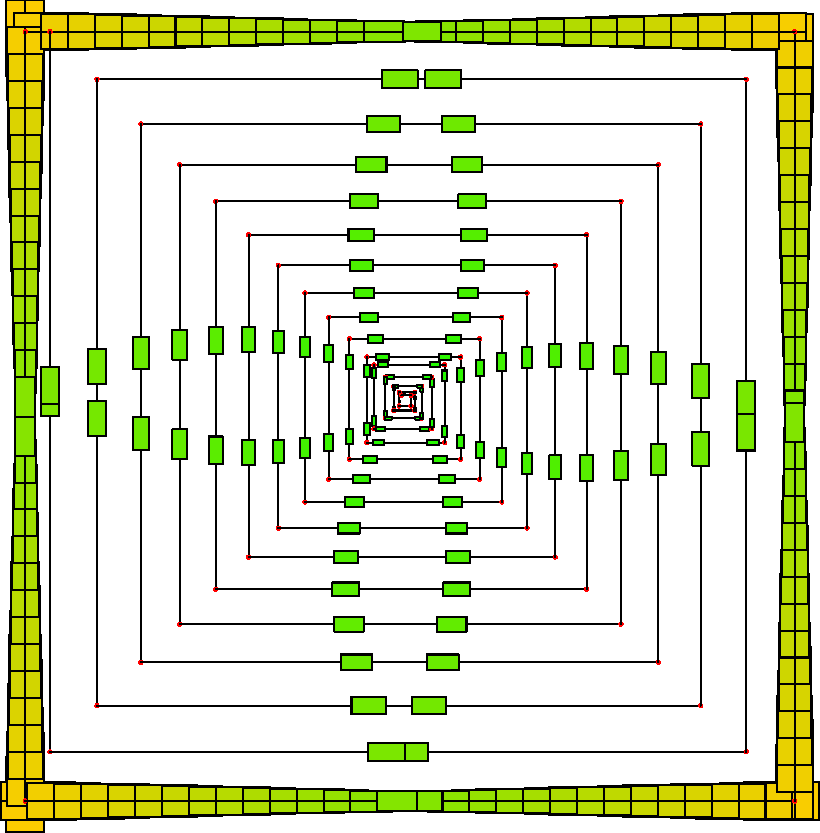
\includegraphics[scale=.5]{./asytopdf/insolite2.pdf}
\end{center}

%%%%%%%%%%%%%%%%%%%%%%%%%%%%%%
\end{document}
%%%%%%%%%%%%%%%%%%%%%%%%%%%%%%



